Obvious is a set of interfaces and extension classes for wrapping
around existing information visualization toolkits.  It generalizes
and extends the standard architecture as defined in the Information
Visualization reference model to try to abstract all the existing
implementations.  In this section, we list all of the existing
toolkits and explain what is common and how they differ.  In the
second section, we describe the most common standardization processes
for software systems.

\subsection{Visualization Toolkits}

Mostly all the existing information visualization toolkits follow the
InfoVis reference model initially specified by Ed Chi and refined by
Card, Mackinlay and Shneiderman~\cite{ChiRefModel,ReadingsIV}.  The
model defines three stages: Data Table, Visual Structure and View
(Figure~\ref{fig:refmodel}).  One of its main benefits is that it
explicitly represents interaction, in contrast to older visualization models.
Several articles have described the concrete design of an information
visualization toolkit.  We report here on the common and the
specific parts.

The InfoVis Toolkit~\cite{InfoVis} is based on an \emph{in-memory
  database manager} where data is organized in columns --- contrary to
most relational databases --- to improve the memory footprint and
allow addition of new attributes that are needed to manage the interaction
(e.g. selection or filtering) and to hold attributes computed on
demand.  The main challenge being the support of interactive
performance for rendering and dynamic queries with a small memory
footprint.  The visual structure is managed using a \emph{monolithic}
architecture~\cite{Polylithic}: each visualization technique is
implemented as a specific class (e.g. ScatterplotVisualization,
ParallelCoordinatesVisualization, TreeVisualization) that performs the
mapping between the data tables and the graphics items to render.
Finally, the view component is the same for each of the visual
structures and takes care of scrolling, zooming, overlaying magic
lenses (e.g. Fisheye or Magic Lenses).   A \emph{notification mechanism}
implements the communication between the data tables and the visual
structure: each time a data table is modified, it notifies all the
registered handlers of the details of the modification. The
interaction is managed by \emph{Interactor} objects that are
associated with the visual structures; the views are generic and
forward interaction managements to the Interactors.  One specific
feature provided by the InfoVis Toolkit is layering: visualization can
be composed on top of each others.  Composite visualizations are
useful to build complex visualization by breaking them into simple
parts. For example, node-link diagrams are split into links managed as
a layer and nodes as another.  Magic lenses and Fisheyes are also
managed as layers on top of other visualizations.

Prefuse~\cite{Prefuse} also relies on an in-memory database with
notification but implements the visual structure using an extension of
the data model (a visual table derives from a data table).  It then
transforms the data into a \emph{polylithic} graphic structures
whereas all the other toolkits use a \emph{monolithic} architecture.
In a polylithic architecture, there is only one component in charge of
all the visual structures.  A visualization object is responsible of
managing a visual structure: it contains visual tables that augment
data tables with graphic attributes (shape, color, etc.)
Visualizations are in charge of computing the layout (assigning a
position and shape to visual items), the graphic attributes and
animations.  Visualizations use a \emph{Renderer} object to actually
display visual items.  Users can control which renderer is used
depending on the visualization and the object itself.  In Prefuse,
data managers, visual managers and views are generic, offering a very
clean interface to the application programmer.  However, as noted by
Bederson at al.~\cite{Polylithic}, polylithic toolkits have a steeper
learning curve than monolithic ones because the polylithic components
do not work out of the box, they always need to be configured.  To
address this issue, Prefuse comes with code samples that simplify the
initial setup.

Building upon their experience in the Prefuse toolkit~\cite{Prefuse},
Heer et Agrawala~\cite{DesignPatternsIV} have derived software design
patterns that are common to information visualization applications and
toolkits. 

Improvise~\cite{Improvise} relies on an in-memory database with
notification that is row-oriented and its visual structures are
monolithic.  The main characteristic of Improvise lies in its
management of coordinated views.  To this aim, it relies on several
design patterns not supported by Prefuse; compared to the other
information visualization toolkits, it adds a coordination component
that is central and extends the notification mechanism implemented
by the InfoVis Toolkit or Prefuse.

\jo{I'm not sure I am convinced of the assertion in the following paragraph. The three toolkits above are described in some detail, not all of which is relevant to other toolkits. Perhaps we should instead abstract their distinct design characters. e.g. Row-oriented vs column oriented; in-memory vs cached database management; monolithic vs polylithic etc. The point being that while they all attempt to achieve similar general aims, their lower-level approach to doing so requires different programming approaches, hence the need for Obvious.}

Other information visualization toolkits can mostly be described using
the three toolkits above, even if they use a different programming
language.  Tulip~\cite{Tulip} is a graph-oriented toolkit programmed in C++ that
uses data tables for vertices and edges, like the InfoVis Toolkit and
Prefuse.  It implements several complex graph layout algorithms and
uses OpenGL for its rendering but the conceptual architecture is
table-based and monolithic.

There are also lower-level toolkits that can be used to build visual
analytics applications.  Two popular families are scene-graph managers
and graph libraries.

\jo{I'm not sure what point is being made here with the discussion of lower level visualization toolkits. Are we asserting that the standardization implied by Obvious is also appropriate for lower level approaches to VA software construction? If so, we need to identify what is lacking in an approach without Obvious as well as demonstrating (later on in the paper) that implementing the Obvious interfaces in lower level visualization environments is both practical and beneficial. An interesting test case might be \emph{Processing} (processing.org). This is, compared to the other examples cited, a very low level approach to visualization software development. However, it is designed for rapid-prototyping, and if it could be easily integrated with Obvious it might provide a nice example of how early prototypes could be transformed into more robust applications using Obvious as the bridge. I'd be happy to write some words on this if you think it fits well with the theme of the paper.}

\subsection{Scene-Graph Managers}

Visual analytics applications can manage their own data structure and
manage the mapping from data to visual structure on their own.  At
this point, they can use scene-graph toolkits to manage the
visual structure and view as described in the reference model.

Scene-graph toolkits are focused on computer graphics and interaction:
they only deal with the visual structure and view.  Piccolo and
Jazz~\cite{Polylithic} are popular 2D scene-graph managers that have
been used to create several information visualization applications
(e.g.~\cite{SpaceTree,Geneaquilt}.) An early version of Piccolo has
also been used as graphics engine for the Cytoscape graph
visualization system~\cite{Cytoscape} but dropped for performance
reasons.

High-performance information visualization applications use
scene-graph optimization techniques to speed-up the rendering of
scenes.  Tulip~\cite{Tulip} and Gephi~\cite{Gephi} maintain a spatial
indexing structure to avoid rendering objects that are not visible.

Although scene-graph technologies are mature and used in a wide
variety of graphics applications such as games, virtual-reality
applications and scientific visualization systems, they are not
adequate for information visualization systems because they require
the explicit specification of geometry and graphic attributes for each
displayed objects.  Very often, information visualization can quickly
compute graphic attribute and even geometry from data attributes.  For
example, the position of an item using a scatterplot visualization is
computed using a simple affine transformation from two data
attributes.  There is no need to store the computed values when
computing them on the fly is very cheap.  The same is true for color
etc.  Copying this information is costly in term of time and memory.

Still, by separating the data-model from the visual model, scene-graph
managers offer more flexibility than information visualization systems
for complex graphics and sophisticated interaction.  This is why
several information visualization systems still use them.


\subsection{Graph Managers}

\jo{Referred to as `graph libraries' above.}

While most table-based visualization toolkits rely on an in-memory
database, several graph-based visualization systems manage their
data-structures using a model inspired from graph-theory where
topology is the main focus and data associated with graph entities is
less important.  This is the case for the JUNG library~\cite{jung2003}
or the Boost Graph Library (BGL)~\cite{BGL}, as well as for the graph
library used by Cytoscape~\cite{Cytoscape}.

These libraries support graphs as set of vertices and edges (the
topological entities) that can be associated with arbitrary data.
This data is just stored by the graph entities as a convenience for
the application: the library does not implement any integrity check
between data and graph entities. ++


\begin{figure}
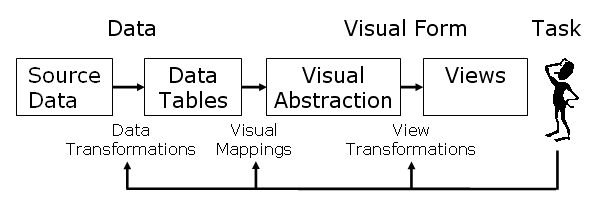
\includegraphics[width=\columnwidth]{figures/reference_model}
\caption{The Information Visualization Reference Model (drawing by
  J. Heer)}
\label{fig:refmodel}
\end{figure}


\subsection{Standardization processes}
ISO, Internet, SQL





